\begin{pages}
    \begin{Rightside}
    \selectlanguage{greek}
        \beginnumbering
        \pstart[
        			\chapter{Ὁ βιβλίον κατεσφραγισμένον}
        			\markboth{The Sealed Book}
				]
		Καὶ εἶδον ἐπὶ τὴν δεξιὰν τοῦ καθημένου ἐπὶ τοῦ θρόνου βιβλίον γεγραμμένον ἔσωθεν καὶ ὄπισθεν, κατεσφραγισμένον σφραγῖσιν ἑπτά. καὶ εἶδον ἄγγελον ἰσχυρὸν κηρύσσοντα ἐν φωνῇ μεγάλῃ Τίς ἄξιος ἀνοῖξαι τὸ βιβλίον καὶ λῦσαι τὰς σφραγῖδας αὐτοῦ; καὶ οὐδεὶς ἐδύνατο ἐν τῷ οὐρανῷ οὐδὲ ἐπὶ τῆς γῆς οὐδὲ ὑποκάτω τῆς γῆς ἀνοῖξαι τὸ βιβλίον οὔτε βλέπειν αὐτό. καὶ ἔκλαιον πολὺ, ὅτι οὐδεὶς ἄξιος εὑρέθη ἀνοῖξαι τὸ βιβλίον οὔτε βλέπειν αὐτό.
		\pend
		\pstart
		καὶ εἷς ἐκ τῶν πρεσβυτέρων λέγει μοι Μὴ κλαῖε· ἰδοὺ ἐνίκησεν ὁ Λέων ὁ ἐκ τῆς φυλῆς Ἰούδα, ἡ Ῥίζα Δαυείδ, ἀνοῖξαι τὸ βιβλίον καὶ τὰς ἑπτὰ σφραγῖδας αὐτοῦ. Καὶ εἶδον ἐν μέσῳ τοῦ θρόνου καὶ τῶν τεσσάρων ζῴων καὶ ἐν μέσῳ τῶν πρεσβυτέρων Ἀρνίον ἑστηκὸς ὡς ἐσφαγμένον, ἔχων κέρατα ἑπτὰ καὶ ὀφθαλμοὺς ἑπτά, οἵ εἰσιν τὰ ἑπτὰ Πνεύματα τοῦ Θεοῦ ἀπεσταλμένοι εἰς πᾶσαν τὴν γῆν. καὶ ἦλθεν καὶ εἴληφεν ἐκ τῆς δεξιᾶς τοῦ καθημένου ἐπὶ τοῦ θρόνου. 
		\pend
		\pstart
		Καὶ ὅτε ἔλαβεν τὸ βιβλίον, τὰ τέσσερα ζῷα καὶ οἱ εἴκοσι τέσσαρες πρεσβύτεροι ἔπεσαν ἐνώπιον τοῦ Ἀρνίου, ἔχοντες ἕκαστος κιθάραν καὶ φιάλας χρυσᾶς γεμούσας θυμιαμάτων, αἵ εἰσιν αἱ προσευχαὶ τῶν ἁγίων. καὶ ᾄδουσιν ᾠδὴν καινὴν λέγοντες Ἄξιος εἶ λαβεῖν τὸ βιβλίον καὶ ἀνοῖξαι τὰς σφραγῖδας αὐτοῦ, ὅτι ἐσφάγης καὶ ἠγόρασας τῷ 	Θεῷ ἐν τῷ αἵματί σου ἐκ πάσης φυλῆς καὶ γλώσσης καὶ λαοῦ καὶ ἔθνους, καὶ ἐποίησας αὐτοὺς τῷ Θεῷ ἡμῶν βασιλείαν καὶ ἱερεῖς, καὶ βασιλεύσουσιν ἐπὶ τῆς γῆς.
		\pend
		\pstart
		καὶ εἶδον, καὶ ἤκουσα φωνὴν ἀγγέλων πολλῶν κύκλῳ τοῦ θρόνου καὶ τῶν ζῴων καὶ τῶν πρεσβυτέρων, καὶ ἦν ὁ ἀριθμὸς αὐτῶν μυριάδες μυριάδων καὶ χιλιάδες χιλιάδων, λέγοντες φωνῇ μεγάλῃ Ἄξιός ἐστιν τὸ Ἀρνίον τὸ ἐσφαγμένον λαβεῖν τὴν δύναμιν καὶ πλοῦτον καὶ σοφίαν καὶ 	ἰσχὺν καὶ τιμὴν καὶ δόξαν καὶ εὐλογίαν. καὶ πᾶν κτίσμα ὃ ἐν τῷ οὐρανῷ καὶ ἐπὶ τῆς γῆς καὶ ὑποκάτω τῆς γῆς καὶ ἐπὶ τῆς θαλάσσης ἐστίν, καὶ τὰ ἐν αὐτοῖς πάντα, ἤκουσα λέγοντας Τῷ καθημένῳ ἐπὶ τῷ θρόνῳ καὶ τῷ Ἀρνίῳ ἡ εὐλογία καὶ ἡ τιμὴ καὶ ἡ δόξα καὶ τὸ κράτος εἰς τοὺς αἰῶνας τῶν αἰώνων. καὶ τὰ τέσσερα ζῷα ἔλεγον Ἀμήν, καὶ οἱ πρεσβύτεροι ἔπεσαν καὶ προσεκύνησαν.
		\pend
        \endnumbering
    \end{Rightside}
    \begin{Leftside}
        \beginnumbering
        \pstart[
        			\chapter{The Sealed Book}
				]
		And I saw a (little) book upon the right hand of Him who sits upon the throne — (and things were) written within (it) and on its back (behind it) — (and it was) sealed with seven seals. And I saw a strong angel, announcing (preaching) in a great voice, “Who is worthy of opening the book and removing its seals?” And nobody was able to open the book — nor look at it —, neither in Heaven (the sky), nor upon the Earth, nor below the Earth. And I cried vehemently, as nobody was found worthy of either opening or looking at the book.
		\pend
		\pstart
		And one of the elders says to me saying, “Do not cry. Look, the Lion of the people of Juda — the Root of David — was victorious in opening the book and tearing off its seals. And I saw a Lamb standing as if slain (and) having seven heads and seven eyes — which are the seven Spirits of God, sent into the entire Earth — in the middle of the throne and (in the midst of) the four creatures and among the elders. And it came (forth) and took the book out of the right hand of Him who sits upon the throne.
		\pend
		\pstart
		And once he took the book, the four creatures and the twenty-four elders fell (to their knees) before the Lamb, each having a guitar and golden vials filled with incense which are the prayers of the holy. And they sing a new song, saying “You are worthy of taking the book and opening its seals, since You were slain and purchased for God with Your blood (some people) from every tribe and tongue and people and nation; and You have made them (to be) a kingdom and priests for our God and they shall rule upon the Earth. 
		\pend
		\pstart
		And I saw and I heard the voice(s) of many angels around the throne and the creatures and the elders; and their number was myriads of myriads and thousands of thousands. (And the voice was) saying in a great voice, “The slain Lamb is worthy of taking the power and richness and wisdom and might and honour and glory and blessing.” And every creature (creation, being) which is in Heaven and upon the Earth and below the Earth and upon the sea I heard saying “Blessing(s) and honour and glory and power to Him who sits upon the throne and to the Lamb — into the eternity of eternities.” And the four creatures said, “Amen”, and the elders fell (to their knees) and prayed.
		\pend
        \endnumbering
    \end{Leftside}

\end{pages} 
\Pages

\clearpage
\thispagestyle{empty}
\null\vfill
\settowidth\longest{\huge\itshape […] and when I turned around I saw}
\begin{center}
\parbox{\longest}{%
  \raggedright{\huge\itshape%
    ``And I saw a (little) book upon the right hand of Him who sits upon the throne — (and things were) written within (it) and on its back (behind it) — (and it was) sealed with seven seals.'' \par\bigskip
  }
  \raggedleft\Large\MakeUppercase{``Apocalyptic Seals'' — Rudolf Steiner (original sketch) \& Clara Hettich (oil on canvas), 1907 – 1911}\par%
}
\vfill\vfill
\clearpage\newpage
\end{center}
\newpage
\thispagestyle{empty}
\begin{center}
	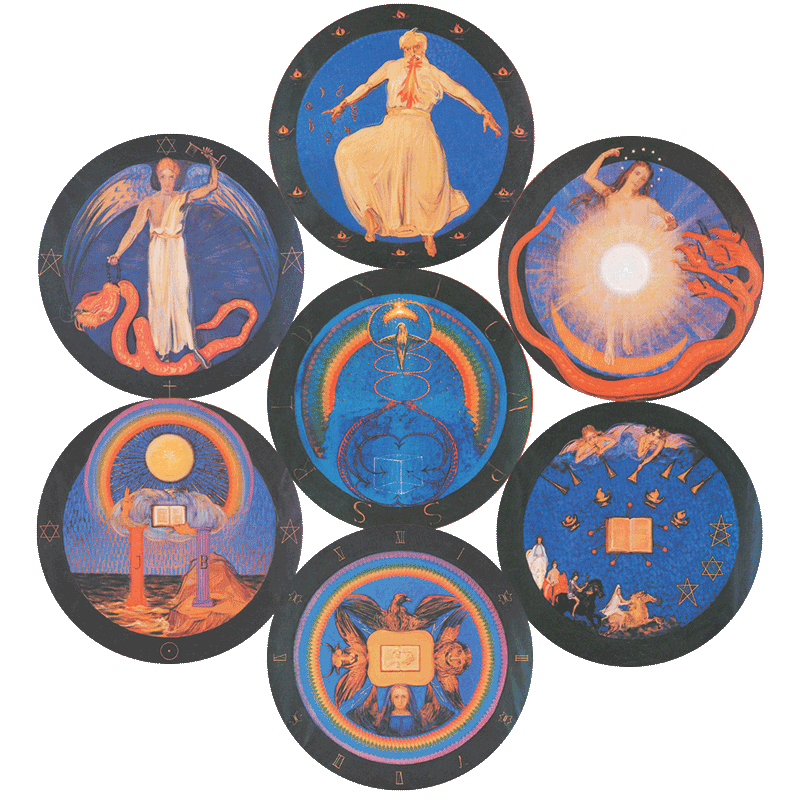
\includegraphics[width=1\textwidth]{images/illustrations/steinerapocalypticseals.png}
\end{center}